% 附录 AG：磁流体平衡与位形（第 33 个附录，v1.26.11 新增）
%
% 数值唯一来源：tools/calc/appAG_calc.py -> tools/calc/appAG_calc.txt
%   （正文里凡标出数字的量都可以在 calc 输出里逐位找到；单位一律写在数学模式内，
%    避免中文字符进入数学字体）
% 速度与几何口径：与附录 AD/AE/AF 同一工作点 R=6.2 m、a=2.0 m、B0=5.3 T、I_p=15 MA、
%   kappa=1.7、delta=0.4、n_e=1e20 m^-3、T_e=T_i=9194 eV、m_i=2.5 m_p。
% 版权口径：只借鉴经典教材与文献的结论、公式形式与题型；文字、数值、表格均自拟并由
%   tools/calc/appAG_calc.py 独立复算。离线环境无法核验 DOI，故只给作者、年份、卷期页。
% 与相邻附录的分工：本附录讲「平衡」（给定压强与电流，磁面长什么样）；磁岛与拓扑留给
%   附录 T，台基与边界稳定性留给附录 AD，输运定标留给附录 S，位形比较留给附录 AA。

\section{磁面与安全因子：嵌套结构是从哪来的}
\label{sec:app-ag-surfaces}

前面几十章里，我们一直把「磁面」当成一个既成事实：磁场把等离子体切成一层层嵌套的
环面，粒子和热量沿着磁面跑得快、穿过磁面跑得慢，于是才有约束。但磁面并不是画出来的，
它是\textbf{平衡方程的解}——压强梯度往外推、电流产生的极向场往里箍，两者在每一条磁面上
刚好抵消，磁面才停在那里。本节先把这套几何语言翻译成几个可以算的数。

第一个数是反宽高比
\begin{equation}
\epsilon = \frac{a}{R} = \frac{2.0}{6.2} = 0.322581,
\label{eq:app-ag-epsilon}
\end{equation}
它衡量「环」得有多厉害：$\epsilon$ 越小，托卡马克越接近一根直螺线管，后面几乎所有
展开式都按 $\epsilon$ 的小量来做。本工作点的 $R/a = 3.1$，属于中等环径比。

第二个数是极向磁场。环向电流 $I_p$ 绕着大环流一圈，在半径 $a$ 处产生的极向场是
\begin{equation}
B_\theta(a) = \frac{\mu_0 I_p}{2\pi a} = \frac{1.2566\times10^{-6}\times15.0\times10^{6}}
{2\pi\times2.0} = 1.5\ \mathrm{T},
\label{eq:app-ag-btheta}
\end{equation}
只有环向场 $5.3\ \mathrm{T}$ 的 $28.3019\%$。可就是这个「小」场决定了磁力线绕大环转多少圈
才回到原处：安全因子
\begin{equation}
q_{\rm cyl} = \frac{a B_0}{R B_\theta(a)} = 1.13978,
\qquad
q_{95} = q_{\rm cyl}\,\frac{1+\kappa^2}{2} = 2.21688,
\label{eq:app-ag-q95}
\end{equation}
其中 $\kappa=1.7$ 是截面伸长比（拉长的椭圆），$q_{95}$ 表示在归一化极向磁通 $95\%$
处的 $q$ 值，是工程上最常引用的那个数。$q_{95}=2.21688$ 意味着磁力线要绕环向
$2.2$ 圈才回到同一根极向位置——这个数太小，正是后面要谈的稳定性隐患。

磁力线上相邻两条磁面之间，剪切有多大？取抛物线型剖面 $q(r)=q_0+(q_{95}-q_0)(r/a)^2$，
边界附近的磁剪切为
\begin{equation}
s_{95} = \frac{2(q_{95}-q_0)}{q_{95}} = 1.09783,
\label{eq:app-ag-shear}
\end{equation}
它和 $q_{95}$ 一起构成稳定性分析的两个输入（附录 T 与 AD 会各用一次）。

几何量同样可以直接点清：环向磁通 $\Phi_{\rm tor}=B_0\pi a^2\kappa = 113.223\ \mathrm{Wb}$，
极向磁通 $\Phi_{\rm pol}=\Phi_{\rm tor}/q_{95}=51.0731\ \mathrm{Wb}$，两者之比就是
安全因子的定义；等离子体体积
\begin{equation}
V = 2\pi^2 R a^2 \kappa = 832.205\ \mathrm{m^3},
\label{eq:app-ag-volume}
\end{equation}
与附录 M/S/Z 用的 $832.2\ \mathrm{m^3}$ 是同一个数——这不是巧合，而是同一个公式；
壁面积按圆柱近似 $S=4\pi^2 R a = 489.532\ \mathrm{m^2}$，也与附录 X 的迎风面积一致。
最后记住环向场的 $1/R$ 衰减：内中平面 $7.82381\ \mathrm{T}$、外中平面 $4.00732\ \mathrm{T}$，
相差接近一倍——这个不对称是后面 Shafranov 位移把磁轴往外推的几何背景。

\begin{table}[htbp]
\centering
\small
\begin{tabular}{p{3.4cm}p{2.9cm}p{4.2cm}p{4.4cm}}
\toprule
量 & 本工作点 & 它从哪里来 & 它决定什么 \\
\midrule
反宽高比 $\epsilon$ & $0.322581$ & $a/R$，几何 & 展开式的小量、环径比 \\
极向场 $B_\theta(a)$ & $1.5\ \mathrm{T}$ & $\mu_0 I_p/(2\pi a)$ & 磁力线的螺距 \\
安全因子 $q_{95}$ & $2.21688$ & 环向磁通与极向磁通之比 & 扭曲模、磁岛、约束 \\
磁剪切 $s_{95}$ & $1.09783$ & $q$ 剖面的斜率 & 局域稳定性判据 \\
体积 $V$ & $832.205\ \mathrm{m^3}$ & $2\pi^2 R a^2 \kappa$ & 功率密度与总储能 \\
\bottomrule
\end{tabular}
\caption{磁面几何的五个基本量。注意它们全部由 $R$、$a$、$B_0$、$I_p$、$\kappa$ 五个输入
导出，没有额外自由参数。}
\label{tab:app-ag-scales}
\end{table}

\begin{tip}{磁面不是画出来的，是平衡方程的解}{tip-app-ag-surfaces}
「嵌套磁面」不是设计者的选择，而是压强梯度和极向场在每一点互相抵消的结果。压强越大、
电流越小，磁面就越会往外挤——第三节的 Shafranov 位移说的就是这件事。
\end{tip}

\textbf{出处：}磁面几何与安全因子的记法参照 Freidberg \emph{Ideal MHD}（2014，第 5--6 章）、
Wesson \emph{Tokamaks}（第 4 版，2011，第 3 章）与 ITER Physics Basis（\emph{Nucl. Fusion}
\textbf{39} (1999) 2137）；本节的写法与全部数值由 \texttt{tools/\allowbreak{}calc/\allowbreak{}appAG\_calc.py} 复算。

\begin{figure}[htbp]
\centering
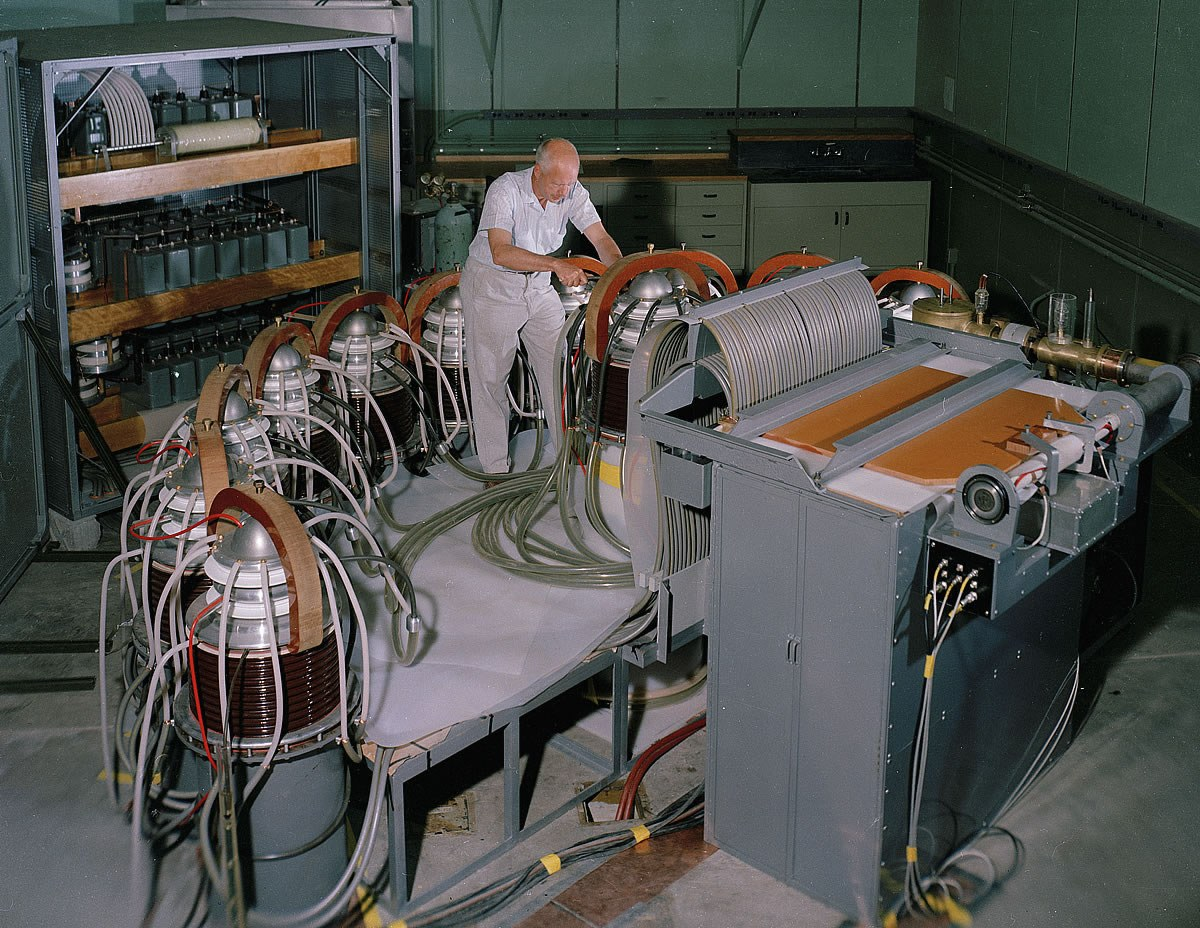
\includegraphics[width=0.78\textwidth]{../figures/scylla_theta_pinch.jpg}
\caption{$\theta$ 箍缩 Scylla I：磁面嵌套最早的实验版本。1958 年的 Scylla I 用一条快速上升的环向电流把等离子体压缩成磁通管，这是「磁面嵌套」最朴素的实现；本书附录 AG 讲的磁面、安全因子与平衡，正是从这类装置的测量里长出来的。}
\label{fig:photo-appag}
\figsource{Unknown LANL photographer，Public domain（Wikimedia Commons）}
\end{figure}

\section{Grad--Shafranov 方程：平衡是压强与电流的两本账}
\label{sec:app-ag-gs}

有了磁面的语言，就可以问那个最基本的问题：给定压强剖面 $p(\psi)$ 和环向场函数
$F(\psi)=RB_\phi$，磁面 $\psi(R,Z)$ 长什么样？答案是一条椭圆型二阶偏微分方程，
即 Grad--Shafranov 方程
\begin{equation}
\Delta^* \psi = -\mu_0 R^2 \frac{dp}{d\psi} - F\frac{dF}{d\psi},
\qquad
\Delta^* \equiv R\frac{\partial}{\partial R}\!\left(\frac{1}{R}\frac{\partial}{\partial R}\right)
+ \frac{\partial^2}{\partial Z^2},
\label{eq:app-ag-gs}
\end{equation}
它看起来唬人，其实就是两本账：右边第一项是\textbf{压强往外推}，第二项是
\textbf{环向场与极向电流往里箍}，左边是磁面的弯曲程度。两者在每条磁面上刚好配平，
磁面才静止不动。

把本工作点代进去，先算两个「账目」的量级。体积平均压强（$n_e=1\times10^{20}\ \mathrm{m^{-3}}$、
$T_e=T_i=9194\ \mathrm{eV}$，两种粒子各半）
\begin{equation}
\langle p\rangle = 2 n_e T_e = 2.94608\times10^{5}\ \mathrm{Pa},
\label{eq:app-ag-pressure}
\end{equation}
压强梯度量级 $|\nabla p|\sim \langle p\rangle/a = 1.47304\times10^{5}\ \mathrm{Pa\,m^{-1}}$，
平均电流密度 $\langle j\rangle = I_p/(\pi a^2\kappa) = 7.02154\times10^{5}\ \mathrm{A\,m^{-2}}$。
两个无量纲的比压随之确定：
\begin{equation}
\beta_t = \frac{2\mu_0\langle p\rangle}{B_0^2} = 0.0263592 = 2.63592\%,
\qquad
\beta_p = \frac{2\mu_0\langle p\rangle}{B_\theta^2(a)} = 0.329081 = 32.9081\%,
\label{eq:app-ag-betat}
\end{equation}
同一团等离子体，对着环向场算只有 $2.63592\%$，对着极向场算却有 $32.9081\%$——因为极向场
本来就只有 $1.5\ \mathrm{T}$。工程上更常用归一化比压
\begin{equation}
\beta_N = \beta_t[\%]\,\frac{a B_0}{I_p[\mathrm{MA}]} = 1.86272,
\label{eq:app-ag-betan}
\end{equation}
它的好处是把 $\beta_t$ 与装置尺寸、电流的依赖打包掉，剩下一个可以和稳定性极限直接
比较的数（第五节）。

方程 (\ref{eq:app-ag-gs}) 里还有一个不显眼但很关键的组合：环向场函数
$F=B_0R = 32.86\ \mathrm{T\,m}$。在低比压极限下 $F\approx$ 常数，于是
$B_\phi\propto 1/R$；一旦比压不可忽略，$F$ 会随磁面变化，正是这个变化把磁轴推离几何中心。
本节只把两本账算清楚，不解方程——数值平衡解（EFIT、VMEC、CHEASE 这类程序）超出本附录
范围。

\begin{table}[htbp]
\centering
\small
\begin{tabular}{p{3.8cm}p{3.0cm}p{3.6cm}p{4.5cm}}
\toprule
量 & 本工作点 & 表达式 & 物理含义 \\
\midrule
$\langle p\rangle$ & $2.94608\times10^{5}\ \mathrm{Pa}$ & $2n_eT_e$ & 往外推的账 \\
$\langle j\rangle$ & $7.02154\times10^{5}\ \mathrm{A\,m^{-2}}$ & $I_p/(\pi a^2\kappa)$ & 往里箍的账 \\
$\beta_t$ & $2.63592\%$ & $2\mu_0\langle p\rangle/B_0^2$ & 对环向场的效率 \\
$\beta_p$ & $32.9081\%$ & $2\mu_0\langle p\rangle/B_\theta^2$ & 对极向场的效率 \\
$\beta_N$ & $1.86272$ & $\beta_t[\%]aB_0/I_p[\mathrm{MA}]$ & 与极限比较的口径 \\
\bottomrule
\end{tabular}
\caption{Grad--Shafranov 方程右边的两本账。$\beta_t$ 与 $\beta_p$ 相差一个
$(B_0/B_\theta)^2 = 12.4844$ 的因子，这个因子后面还会以 Shafranov 位移的形式出现。}
\label{tab:app-ag-gs}
\end{table}

\begin{tip}{Grad--Shafranov 方程不是新物理，是两条账}{tip-app-ag-gs}
左边只描述磁面几何，右边只有两件事：压强梯度往外推、$F\,dF/d\psi$ 往里箍。
把这条方程当成「磁面的力平衡」，比记它的算符形式有用得多。
\end{tip}

\textbf{出处：}Grad--Shafranov 方程的推导与各项含义参照 Grad \& Rubin（1958，第二次
日内瓦会议论文集 \textbf{31}，190）、Shafranov（\emph{Reviews of Plasma Physics}
\textbf{2} (1966) 103）与 Freidberg \emph{Ideal MHD}（2014，第 6、11 章）；
本节的写法与全部数值由 \texttt{tools/\allowbreak{}calc/\allowbreak{}appAG\_calc.py} 复算。

\section{Shafranov 位移：磁轴为什么往外跑}
\label{sec:app-ag-shift}

如果环向场严格按 $1/R$ 衰减、极向场又均匀，磁面应该以几何中心 $R$ 为圆心。但真实
托卡马克的磁轴总是\textbf{往外}（低场侧）偏一点，这个偏移叫 Shafranov 位移。它的大小
可以用小 $\epsilon$ 展开写成著名的
\begin{equation}
\Delta = \frac{a^2}{2R}\left(\beta_p + \frac{l_i}{2}\right)
= \frac{2.0^2}{2\times6.2}\left(0.329081 + 0.5\right) = 0.267445\ \mathrm{m},
\label{eq:app-ag-shift}
\end{equation}
其中 $l_i=1.0$ 是电流剖面的内电感（声明值，代表电流在截面上有多「尖」）。位移占小半径的
\begin{equation}
\frac{\Delta}{a} = 0.133723 = 13.3723\%,
\label{eq:app-ag-gap}
\end{equation}
放在 $R$ 上就是磁轴位置 $R_{\rm axis} = R+\Delta = 6.46745\ \mathrm{m}$，轴心环向场因此
降到 $B_0R/R_{\rm axis} = 5.08083\ \mathrm{T}$——位移自己又把场降了一点，这是一个
自洽的小回路。

位移的后果很实在：内外侧的磁面间距不再相等。内侧只剩 $a-\Delta = 1.73255\ \mathrm{m}$，
外侧涨到 $a+\Delta = 2.26745\ \mathrm{m}$，比值
\begin{equation}
\frac{a+\Delta}{a-\Delta} = 1.30873.
\label{eq:app-ag-axis}
\end{equation}
也就是说，同样一圈磁通，在外侧占的地方比内侧多三成。这对偏滤器、射频天线的位置和
中子壁负载都有影响（附录 N、M、Z 各用一次）。

位移还有一个「安全阀」的读法：$\Delta$ 随 $\beta_p$ 线性增长，而 $\beta_p\propto 1/B_\theta^2
\propto 1/I_p^2$。要跑到 $\Delta=a/2=1.0\ \mathrm{m}$（磁轴跑到等离子体边缘），需要
$\beta_p = 2.6$，是本工作点 $0.329081$ 的将近八倍——所以环径比越大、电流越足的装置，
越不容易被位移吃掉。反过来，$\beta_p$ 翻倍时 $\Delta$ 从 $0.267445\ \mathrm{m}$ 涨到
$0.3736\ \mathrm{m}$，代价立刻可见。

\begin{table}[htbp]
\centering
\small
\begin{tabular}{p{4.0cm}p{3.0cm}p{3.6cm}p{4.2cm}}
\toprule
量 & 本工作点 & 表达式 & 后果 \\
\midrule
$\Delta$ & $0.267445\ \mathrm{m}$ & $(a^2/2R)(\beta_p+l_i/2)$ & 磁轴外移 \\
$\Delta/a$ & $13.3723\%$ & 相对小半径 & 内外间距不对称 \\
$R_{\rm axis}$ & $6.46745\ \mathrm{m}$ & $R+\Delta$ & 轴心场降到 $5.08083\ \mathrm{T}$ \\
$(a+\Delta)/(a-\Delta)$ & $1.30873$ & 内外间距比 & 偏滤器与壁负载 \\
$\Delta=a/2$ 所需 $\beta_p$ & $2.6$ & 反解 & 大电流装置更安全 \\
\bottomrule
\end{tabular}
\caption{Shafranov 位移的四个读数。位移不是误差，而是压强与电流付的账；它把「比压」
从稳定性问题变成了几何问题。}
\label{tab:app-ag-shift}
\end{table}

\begin{tip}{位移不是误差，是压强与电流付的账}{tip-app-ag-shift}
$\Delta\propto(\beta_p+l_i/2)$：压强越大、电流越尖，磁轴越往外跑。$\Delta$ 与
$1/I_p^2$ 成正比，所以提高电流既压住位移，又顺带抬高 $q$ 的余量——这就是大电流
装置在设计上诱人的地方。
\end{tip}

\textbf{出处：}Shafranov 位移的小 $\epsilon$ 表达式参照 Shafranov（\emph{Reviews of
Plasma Physics} \textbf{2} (1966) 103）、Zakharov \& Shafranov（\emph{Sov. Phys.
Tech. Phys.} \textbf{18} (1973) 151）与 Wesson \emph{Tokamaks}（第 4 版，2011，
第 3 章）；本节的写法与全部数值由 \texttt{tools/\allowbreak{}calc/\allowbreak{}appAG\_calc.py} 复算。
\begin{figure}[htbp]
\centering
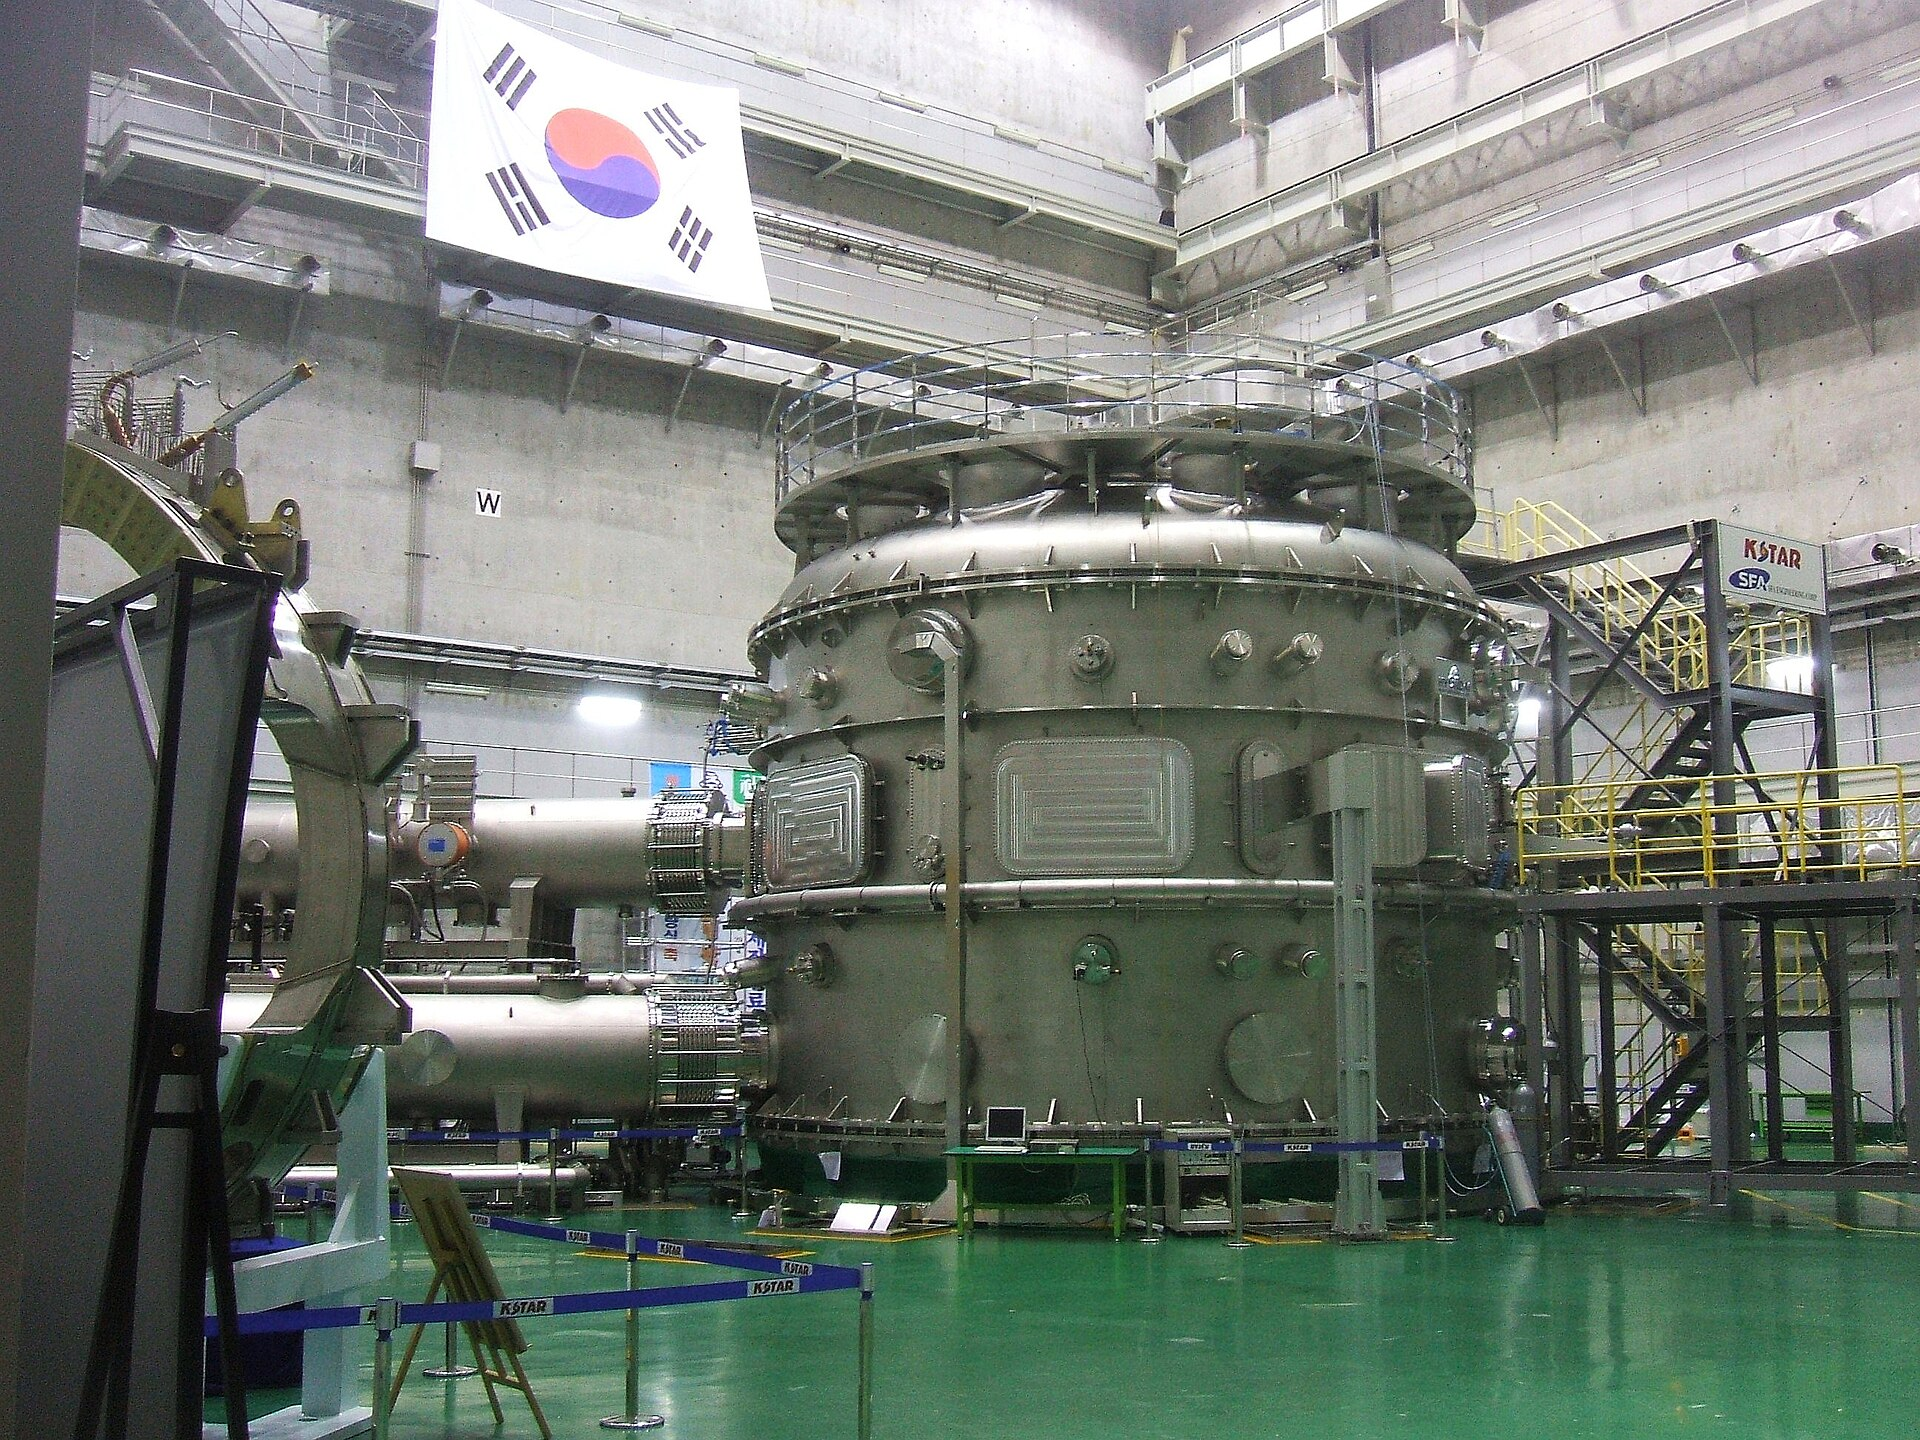
\includegraphics[width=0.78\textwidth]{../figures/ag_kstar_tokamak.jpg}
\caption{把等离子体拉长、压成 D 形，是为了在同样磁场下多装压强与电流。图为 KSTAR 装置本体与厂房：等离子体就装在中间那个环形真空室里，外面一圈 shaping 线圈，正是本节伸长比 $\kappa$ 与三角形变 $\delta$ 的实物落点。}
\label{fig:photo-appag3}
\figsource{Eye Steel Film，CC BY 2.0（Wikimedia Commons）}
\end{figure}

\section{位形参数：伸长比与三角形变买到了什么}
\label{sec:app-ag-shaping}

第一节里出现过一个不太起眼的因子 $(1+\kappa^2)/2$，它就是「形状」在平衡里的价格标签。
对同样的小半径和环向场，安全因子与电流成反比，而形状因子把这条关系改写成
\begin{equation}
q_{95} \simeq \frac{2\pi a^2 B_0}{\mu_0 R I_p}\,\frac{1+\kappa^2}{2}
\quad\Longrightarrow\quad
I_p^{\max} \propto \frac{1+\kappa^2}{2}.
\label{eq:app-ag-shape}
\end{equation}
换句话说：\textbf{把截面拉长并不改变磁场，它买到的是电流}。本工作点 $\kappa=1.7$ 给出的
形状因子是 $1.945$；如果截面是圆的，同样的 $q_{95}$ 只能通
$7.71208\ \mathrm{MA}$，而现在通 $15\ \mathrm{MA}$。反过来，若把 $\kappa$ 提到 $2.0$，
同样 $q_{95}$ 下可以通
\begin{equation}
I_p^{\max}(\kappa=2.0) = 19.2802\ \mathrm{MA},
\qquad
I_p^{\max}(\kappa=1.3) = 10.3728\ \mathrm{MA}.
\label{eq:app-ag-current}
\end{equation}
这条式子解释了一个工程事实：现代托卡马克都是「竖着的椭圆」，不是审美问题，而是
在 $q_{95}$ 这条安全线以下多要几兆安培的电流。

三角形变 $\delta$ 买的是另一样东西。它几乎不影响 $q_{95}$，却改变了磁面的局域曲率，
把气球模的驱动压低：本工作点取 $\delta=0.4$，稳定性计算（附录 AD）里把比压极限提高了
$20\%$（声明值，取自文献的经验区间）。面积与体积对形状的响应也能一眼看出：
体积 $V=2\pi^2 R a^2\kappa$ 对 $a$ 是平方、对 $\kappa$ 是线性。若把 $a$ 放大 $10\%$、
$R$ 放大 $5\%$，体积从 $832.205\ \mathrm{m^3}$ 涨到 $1057.32\ \mathrm{m^3}$——多出来的
每一立方米都要靠磁场去约束。

\begin{table}[htbp]
\centering
\small
\begin{tabular}{p{2.4cm}p{2.6cm}p{3.4cm}p{3.6cm}p{2.6cm}}
\toprule
伸长比 $\kappa$ & 形状因子 & 同样 $q_{95}$ 允许的 $I_p$ & 相对圆截面 & 说明 \\
\midrule
$1.0$ & $1.0$ & $7.71208\ \mathrm{MA}$ & $1.0$ 倍 & 圆截面基准 \\
$1.3$ & $1.345$ & $10.3728\ \mathrm{MA}$ & $1.345$ 倍 & 早期装置 \\
$1.7$ & $1.945$ & $15.0\ \mathrm{MA}$ & $1.945$ 倍 & 本工作点 \\
$2.0$ & $2.5$ & $19.2802\ \mathrm{MA}$ & $2.5$ 倍 & 形状的极限一侧 \\
\bottomrule
\end{tabular}
\caption{伸长比的「汇率」：$(1+\kappa^2)/2$ 就是同样安全因子下能多通多少电流。
$\kappa$ 不能无限拉——拉得越长，垂直位移不稳定（附录 AA、V）越难控制。}
\label{tab:app-ag-shaping}
\end{table}

\begin{tip}{伸长比不是造型，是买电流}{tip-app-ag-shaping}
$(1+\kappa^2)/2$ 出现在 $q_{95}$ 的分母里，所以拉长截面等于给电流「打折」。
$\kappa=1.7$ 相对圆截面多要了将近一倍的电流，代价是垂直稳定性必须靠反馈控制兜住。
\end{tip}

\textbf{出处：}形状因子与 $\beta_N$ 的三角形变增益参照 Troyon 等（\emph{Plasma Phys.
Control. Fusion} \textbf{26} (1984) 209）、Freidberg \emph{Ideal MHD}（2014，第 6、12 章）
与 ITER Physics Basis（\emph{Nucl. Fusion} \textbf{39} (1999) 2137）；本节的写法与
全部数值由 \texttt{tools/\allowbreak{}calc/\allowbreak{}appAG\_calc.py} 复算。

\section{压强极限：比压能推到多高}
\label{sec:app-ag-beta}

比压 $\beta$ 是「用磁场换聚变功率」的效率：$\beta$ 越大，同样磁场下能装的压强越多，
聚变功率密度越高。但它有上限，而这个上限不是材料强度给的，是\textbf{磁场的刚度}给的——
磁压 $B^2/2\mu_0$ 必须远大于等离子体压强，否则磁面自己就被推散了。

先看量级上界。由维里定理可以证明，环向比压受 $\epsilon/q^2$ 量级的限制，
本工作点
\begin{equation}
\frac{\epsilon}{q_{95}^2} = 0.0656377 = 6.56377\%,
\label{eq:app-ag-virial}
\end{equation}
而实际用了 $2.63592\%$，只有它的四成。工程上更常引用的是 Troyon 型经验极限
\begin{equation}
\beta_N \lesssim 3.0
\quad\Longrightarrow\quad
\beta_t^{\max} = 4.24528\%,
\qquad
\langle p\rangle^{\max} = 4.74481\times10^{5}\ \mathrm{Pa}.
\label{eq:app-ag-troyon}
\end{equation}
本工作点 $\beta_N=1.86272$，只用了极限的 $62.0907\%$——也就是说，如果稳定性允许，
还可以把压强提高约六成，聚变功率密度大致按 $\langle p\rangle^2$ 上涨。

代价立刻从平衡里读出来。把 $q_{95}$ 抬到 $3.0$（扭曲模的常规安全线），需要把电流降到
\begin{equation}
I_p(q_{95}=3.0) = \frac{2\pi a^2 B_0}{\mu_0 R q_{95}}\frac{1+\kappa^2}{2}
= 11.0844\ \mathrm{MA},
\label{eq:app-ag-alpha}
\end{equation}
比现在低 $1.35325$ 倍。电流一降，Greenwald 密度也跟着降：$n_G = 8.82069\times10^{19}\ \mathrm{m^{-3}}$，
于是 $n_e/n_G = 1.1337>1$——工作点反而\textbf{越过了密度极限}。这组数把聚变堆设计的
两难说得很清楚：\textbf{$q_{95}$ 的安全线、Greenwald 密度线、以及 $\beta$ 的效率线，
三条线不能同时舒服地满足}，只能各自留余量。本附录的做法是把这组矛盾原样摆出来，
而不是假装它不存在。

最后给出一个局域量，供第六节与附录 AD 衔接：压强梯度驱动的气球模参数
\begin{equation}
\alpha = \frac{2\mu_0 q_{95}^2 R \langle p\rangle}{a B_0^2} = 0.401587,
\label{eq:app-ag-mercier}
\end{equation}
与附录 AD 里台基处用的 $\alpha_{\rm crit}=2.5$ 相比只有 $0.160635$——可见芯部的
气球模驱动远小于台基，稳定性问题主要集中在边上那十几厘米。

\begin{table}[htbp]
\centering
\small
\begin{tabular}{p{3.4cm}p{3.0cm}p{2.8cm}p{4.4cm}}
\toprule
量 & 本工作点 & 极限或对照 & 余量 \\
\midrule
$\beta_t$ & $2.63592\%$ & $4.24528\%$（$\beta_N=3$） & 用了 $62.0907\%$ \\
$\langle p\rangle$ & $2.94608\times10^{5}\ \mathrm{Pa}$ & $4.74481\times10^{5}\ \mathrm{Pa}$ & 可再涨六成 \\
$\epsilon/q_{95}^2$ & $6.56377\%$ & 维里量级上界 & 用了四成 \\
$q_{95}$ & $2.21688$ & $3.0$（安全线） & 偏低，需降流 \\
$n_e/n_G$ & $0.85$（附录 AD 口径） & $1.0$ & 降流后变成 $1.1337$ \\
\bottomrule
\end{tabular}
\caption{三条线互相拉扯：比压要效率、安全因子要余量、密度要低于 Greenwald 线。
本工作点在 $q_{95}$ 上偏紧，在比压上偏松——这正是聚变堆设计的自由度所在。}
\label{tab:app-ag-beta}
\end{table}

\begin{tip}{比压的上限不是材料强度，是磁场的刚度}{tip-app-ag-beta}
$\beta$ 上不去，不是因为容器会被压坏，而是因为磁压不够把等离子体压强箍住。
维里量级 $\epsilon/q_{95}^2$ 与 Troyon 极限 $\beta_N\lesssim3$ 是两把不同的尺子，
前者是理论量级，后者是实验归纳，用哪一个要说明口径。
\end{tip}

\textbf{出处：}维里定理与比压量级上界参照 Greene, Johnson \& Weimer（\emph{Phys.
Fluids} \textbf{14} (1971) 671）与 Freidberg \emph{Ideal MHD}（2014，第 11--12 章）；
Troyon 型极限与形状增益取自 Troyon 等（\emph{Plasma Phys. Control. Fusion} \textbf{26}
(1984) 209）、Wesson \emph{Tokamaks}（第 4 版，2011，第 3、6 章）与 ITER Physics Basis
（\emph{Nucl. Fusion} \textbf{39} (1999) 2137）；本节的写法与全部数值由
\texttt{tools/\allowbreak{}calc/\allowbreak{}appAG\_calc.py} 复算。

\section{从平衡到稳定性：与磁岛、台基的分工}
\label{sec:app-ag-stability}

讲了半天平衡，还没回答那个读者最关心的问题：这个平衡\textbf{能不能待住}？本附录只把
稳定性需要的几个输入算出来，判断留给别的附录——这是刻意的分工，因为稳定性理论本身
（能量原理、扭曲模与撕裂模、气球模与剥离模）足够再写一个附录。

平衡交出去的第一组输入是安全因子剖面：$q_0=1.0$、$q_{95}=2.21688$，
比值 $q_{95}/q_0 = 2.21688$；第二组是磁剪切 $s_{95}=1.09783$。把剪切代进
两个经典判据的量级形式，得到
\begin{equation}
\frac{s_{95}^2}{8} = 0.150654\ (\text{Suydam 型}),
\qquad
\frac{s_{95}^2}{2} = 0.602617\ (\text{Mercier 型}),
\label{eq:app-ag-suydam}
\end{equation}
它们说明：剪切越大，局域判据越容易满足；但剪切太大又会让撕裂模更容易长出来——
这就是为什么 $q$ 剖面要「平一点但不要太平」。

第三组输入是电流剖面的内电感 $l_i=1.0$ 与极向比压的组合
$\beta_p + l_i/2 = 0.829081$，它既决定 Shafranov 位移，也决定外部扭曲模的驱动。
第四组是前面算过的气球模参数 $\alpha=0.401587$：芯部远低于台基的临界值
（附录 AD 的 $\alpha/\alpha_{\rm crit}=1.31084$ 与 $0.819273$，分别对应无自举与含自举），
这说明\textbf{整个装置的稳定性预算，主要花在边界那十几厘米上}（附录 AD 的台基宽度
$1.2\ \mathrm{cm}$、香蕉宽度 $2.54715\ \mathrm{cm}$ 都是同一批数）。

把这些输入排成表，就是本附录要交给后续章节的「接口」：平衡给出背景场与剖面，
稳定性给出这些剖面能撑多久，输运给出撑不住时漏多快（附录 S、AF）。

\begin{table}[htbp]
\centering
\small
\begin{tabular}{p{3.6cm}p{2.8cm}p{3.2cm}p{4.0cm}}
\toprule
平衡输出 & 本工作点 & 交给谁 & 用来判断什么 \\
\midrule
$q_0$、$q_{95}$ & $1.0$、$2.21688$ & 附录 T & 磁岛位置与宽度 \\
$s_{95}$ & $1.09783$ & 附录 T、AD & 局域稳定性判据 \\
$l_i$ & $1.0$ & 附录 V & 外部扭曲模、破裂 \\
$\alpha$ & $0.401587$ & 附录 AD & 气球模驱动 \\
$\beta_p+l_i/2$ & $0.829081$ & 本附录、附录 AA & Shafranov 位移 \\
\bottomrule
\end{tabular}
\caption{平衡交给稳定性与输运的五个接口。本附录只负责把它们算准、把口径写清，
不替后面的附录下结论。}
\label{tab:app-ag-stability}
\end{table}

\begin{tip}{平衡给的是背景，稳定性才说能不能待住}{tip-app-ag-stability}
一条平衡曲线可以很漂亮，却完全不稳定。本附录给出的 $q$、$s$、$l_i$、$\alpha$ 是
稳定性分析的输入，不是结论；把它们当成「能跑」的证据是最常见的误读。
\end{tip}

\textbf{出处：}Suydam 判据参照 Suydam（1958，第二次日内瓦会议论文集 \textbf{31}，157）、
Mercier 判据参照 Mercier（\emph{Nucl. Fusion} \textbf{4} (1964) 213）、能量原理的
系统叙述参照 Freidberg \emph{Ideal MHD}（2014，第 8--11 章）与 Wesson \emph{Tokamaks}
（第 4 版，2011，第 6 章）；本节的写法与全部数值由 \texttt{tools/\allowbreak{}calc/\allowbreak{}appAG\_calc.py} 复算。
\section{估算练习}
\label{sec:app-ag-problems}


\textbf{练习 1}（换一台机器）一台中等装置取 $R=5.5\ \mathrm{m}$、$a=1.5\ \mathrm{m}$、
$B_0=5.3\ \mathrm{T}$、$I_p=8\ \mathrm{MA}$、$\kappa=1.6$，等离子体
$n_e=0.8\times10^{20}\ \mathrm{m^{-3}}$、$T_e=T_i=8\ \mathrm{keV}$。求 $\epsilon$、
$B_\theta(a)$、$q_{95}$、$\beta_t$、$\beta_p$、Shafranov 位移 $\Delta$ 与 $\Delta/a$。

\textbf{练习 2}（形状的价格）同样的小半径、环向场与 $q_{95}$，把截面从圆
（$\kappa=1.0$）拉成 $\kappa=2.0$，允许的环向电流变成几倍？

\textbf{练习 3}（位移的几何后果）用本工作点的 $\Delta=0.267445\ \mathrm{m}$ 与
$a=2.0\ \mathrm{m}$，求外侧磁面间距与内侧磁面间距相对 $a$ 的倍数。

\textbf{练习 4}（体积账）一台装置取 $R=6.5\ \mathrm{m}$、$a=2.2\ \mathrm{m}$、
$\kappa=1.8$，求等离子体体积；与附录 M/S/Z 用的 $832.205\ \mathrm{m^3}$ 相比大了多少。

\textbf{练习 5}（比压的钱）若 $\beta_N=3.0$，在 $I_p=15\ \mathrm{MA}$、$a=2.0\ \mathrm{m}$、
$B_0=5.3\ \mathrm{T}$ 下允许的体积平均压强是多少？比本工作点高多少？

\textbf{练习 6}（三条线的冲突）把 $q_{95}$ 抬到 $3.0$，需要把电流降到多少？此时
Greenwald 密度变成多少，工作点 $n_e=1\times10^{20}\ \mathrm{m^{-3}}$ 的
$n_e/n_G$ 变成多少？

\textbf{解答 1}$\epsilon=0.272727$、$B_\theta=1.06667\ \mathrm{T}$、$q_{95}=2.4121$、
$\beta_t=1.83488\%$、$\beta_p=0.453005$、$\Delta=0.194933\ \mathrm{m}$、
$\Delta/a=12.9955\%$。注意环径比小了（$R/a=3.66667$），位移占比反而略降。

\textbf{解答 2}$2.5$ 倍。因为 $(1+\kappa^2)/2$ 从 $1.0$ 涨到 $2.5$，而 $q_{95}\propto
I_p^{-1}$，所以同样 $q_{95}$ 下电流上限按 $2.5$ 倍放大。

\textbf{解答 3}外侧 $1.13372$ 倍、内侧 $0.866277$ 倍——两侧加起来仍是 $2a$，
但磁通在外侧摊得更开，这就是偏滤器与天线要按外侧设计的原因。

\textbf{解答 4}$V=1117.79\ \mathrm{m^3}$，是 $832.205\ \mathrm{m^3}$ 的 $1.34317$ 倍。
多出来的体积要用同样的磁场去约束，功率密度因此被摊薄。

\textbf{解答 5}$\langle p\rangle^{\max}=4.74481\times10^{5}\ \mathrm{Pa}$，是本工作点
$2.94608\times10^{5}\ \mathrm{Pa}$ 的 $1.61055$ 倍；由于聚变功率密度大致按
$\langle p\rangle^2$ 走，功率密度还能涨到两倍半左右。

\textbf{解答 6}$I_p=11.0844\ \mathrm{MA}$，比现在低 $1.35325$ 倍；$n_G$ 降到
$8.82069\times10^{19}\ \mathrm{m^{-3}}$，于是 $n_e/n_G=1.1337$——超过了密度极限。
这正是第五节说的「三条线不能同时满足」。

\section{来源、分级与版权说明}
\label{sec:app-ag-source}

本附录的数值分三级，读的时候请看清哪一级。

\textbf{第一级：现算级。}凡在正文里标出数字、并在句尾注明由
\texttt{tools/\allowbreak{}calc/\allowbreak{}appAG\_calc.py} 复算的量，都是第一级。它们全部由上表列出的五个几何输入
（$R$、$a$、$B_0$、$I_p$、$\kappa$）与两个剖面参数（$q_0$、$l_i$）导出，可以被逐位复现。
交叉核对脚本 \texttt{tools/\allowbreak{}calc/\allowbreak{}appAG\_check.py} 会把正文里的每个数字与脚本输出比对，
阈值取相对误差 $10^{-3}$。

\textbf{第二级：声明级。}以下量在脚本顶部以输入形式声明，它们的取值属于工程惯例而非
本附录推出：伸长比 $\kappa=1.7$ 与三角形变 $\delta=0.4$；内电感 $l_i=1.0$；轴心安全因子
$q_0=1.0$；$\beta_N$ 上限 $3.0$；三角形变带来的比压增益 $20\%$；壁面积用的圆柱近似
$S=4\pi^2Ra$。凡用到处都写明「声明值」。

\textbf{第三级：文献级。}只作量级对照、不参与结论的：Troyon 极限在文献中的散布区间
（约 $2.8$--$3.5$）、ITER 类装置的 $\beta_N$ 实测水平（约 $1.8$）、
以及数值平衡程序的名称与用途（EFIT、VMEC、CHEASE）。这些量本附录不复算，也不作为
任何数字结论的依据。

\textbf{版权口径。}（1）不复制任何原书的文字、编号、插图与数据表；本附录的文字、
表格与数值均自拟，并由脚本独立复算。（2）不复制文献中的平衡解算例与程序输出图；
EFIT、VMEC、CHEASE 只提及名称与用途，不转载其结果。（3）不复制其他教材的习题；
六道练习与解答均为自拟，且答案全部由脚本给出。（4）离线环境无法核验 DOI，因此
只给作者、年份、卷期页，不引用预印本编号与网络资源。

\textbf{与相邻附录的分工。}本附录讲平衡：给定压强与电流，磁面是什么形状、磁轴偏多少、
比压能到多高。磁岛与拓扑（附录 T）、台基与边界稳定性（附录 AD）、破裂与逃逸
（附录 V）、输运定标（附录 S、AF）、位形比较（附录 AA）、数值方法（附录 AC）各讲一段，
读者按需跳转即可。

\begin{table}[htbp]
\centering
\small
\begin{tabular}{p{3.2cm}p{4.0cm}p{4.4cm}}
\toprule
级别 & 典型量 & 使用规则 \\
\midrule
现算级 & 磁面几何、$\beta$ 三种口径、位移、电流极限 & 可作结论，句尾注明脚本 \\
声明级 & $\kappa$、$\delta$、$l_i$、$q_0$、$\beta_N$ 上限、形状增益 & 只作输入，正文写明「声明值」 \\
文献级 & Troyon 散布、ITER 水平、平衡程序 & 只作量级对照，不作结论 \\
\bottomrule
\end{tabular}
\caption{数值分级。第三级的量在本附录只作量级对照，不作为结论使用。}
\label{tab:app-ag-source}
\end{table}

\begin{tip}{本附录不给什么}{tip-app-ag-honest}
不给数值平衡解（不解 Grad--Shafranov 方程，只算它的两本账），不给稳定性证明
（只交 $q$、$s$、$l_i$、$\alpha$ 四个接口），不给剖面演化的时间行为。
把「平衡成立」与「能待住」分开，是本附录与附录 T、AD 的分工所在。
\end{tip}

\textbf{出处：}本附录的写法参照 Freidberg \emph{Ideal MHD}（2014，第 5--6、11--12 章）、
Wesson \emph{Tokamaks}（第 4 版，2011，第 3、6 章）、Grad \& Rubin（1958，第二次日内瓦
会议论文集 \textbf{31}，190）、Shafranov（\emph{Reviews of Plasma Physics} \textbf{2}
(1966) 103）、Troyon 等（\emph{Plasma Phys. Control. Fusion} \textbf{26} (1984) 209）
与 ITER Physics Basis（\emph{Nucl. Fusion} \textbf{39} (1999) 2137）；数值平衡程序的
名称与用途参照 Lao 等（\emph{Nucl. Fusion} \textbf{25} (1985) 1611）、Hirshman \&
Whitson（\emph{Phys. Fluids} \textbf{26} (1983) 3553）与 Lütjens, Bondeson \& Sauter
（\emph{Comput. Phys. Commun.} \textbf{97} (1996) 219）。本节的写法与全部数值由
\texttt{tools/\allowbreak{}calc/\allowbreak{}appAG\_calc.py} 复算。
